\section{Comparación de preferencias}

25,En esta sección se presentan algoritmos que cumplen:
\begin{description}
	\item[Entrada:] Vector de enteros \texttt{v} y su tamaño \texttt{n}
	\item[Salida:] Entero no negativo que indica el número de pares $i,j$ de posiciones del vector tales que $i < j$ y $v[i] > v[j]$
\end{description}

Es decir, estos algoritmos deberán contar el número de elementos que se encuentran invertidos en el vector.

\subsection{Algoritmo obvio}

El algoritmo que hemos considerado \textbf{obvio} para comprobar el número de inversiones es el siguiente, que simplemente comprueba todas las parejas posibles de elementos del vector y añade $1$ a un contador para cada pareja invertida, devolviendo el valor del contador al final de la ejecución. Esta es su implementación en C++:

\lstinputlisting[firstline=24, lastline=32]{cpps/preferencias.cpp}

El contenido del bucle interno se ejecuta:
\[\sum_{i=0}^{n-2} n-i-1 = \frac{n^2}{2}-\frac{n}{2}\]
veces, por lo que, dado que la inicialización y actualización del bucle y las condiciones comprobadas se realizan en un tiempo constante, es un algoritmo de orden de eficiencia $O(n^2)$.

\subsection{Inversiones y algoritmos de ordenación: Divide y Vencerás}

No pudimos evitar darnos cuenta de la proximidad de nuestro problema con la ordenación de datos. Al ordenar datos, se deshacen las inversiones, y si hay un algoritmo de ordenación que facilite seguir la pista al proceso de deshacer inversiones, podemos aprovecharlo para contar el número de inversiones efectuado.
Por ello buscamos un algoritmo de ordenación con un orden de eficiencia mejor que el del algoritmo obvio (cuadrático) que se pareciese lo máximo posible a nuestro problema. \\

El primer candidato fue el \textit{quicksort} por su rapidez. Sin embargo, no es adecuado para ayudarnos con esta cuestión, pues presenta un comportamiento difícil de controlar en cuanto a inversiones, dado que puede añadir inversiones en el proceso.

A continuación analizamos el algoritmo \textit{heapsort} dado que nos pareció que las propiedades del \textit{heap}, un árbol parcialmente ordenado, podrían arrojar algo de luz al problema; aunque al final resultó que precisamente la estructura de árbol lo hacía un inadecuado candidato.

Por último llego el turno del \textit{mergesort}. Este algoritmo divide el vector original en subvectores, combinando las soluciones. Pero tiene una forma de hacerlo más simple que el resto: tanto en el caso base (en el que se usará inserción) como en la mezcla de vectores podemos controlar el número de inversiones deshechas. \\

Por debajo de un cierto umbral aplicamos el algoritmo de ordenación por inserción, un algoritmo que en cada uno de sus pasos deshace una inversión, por lo que puede usarse este mismo algoritmo para contar el número de inversiones con una variable que se incremente a cada inversión realizada. Resulta más rápido que el algoritmo trivial en este menester, pero sigue siendo $O(n^2)$, y, curiosamente, al usar optimización se invierten los papeles y el algoritmo trivial es más rápido que el algoritmo de inserción. \\

A la hora de mezclar vectores también puede controlarse el número de inversiones deshechas. Consideremos un vector $T$, lo partimos en dos y aplicamos inserción a cada una de sus partes: izquierda ($U$) y derecha ($V$). Se observa que, al ordenar cada parte, las inversiones de los elementos de una parte respecto de elementos de la otra se conservan. Por ello, si en la mezcla de dos vectores $U$ y $V$ se inserta un elemento de $V$ cuando quedan $k$ elementos de $U$ por insertar, se estarán deshaciendo $k$ inversiones. Entonces el número de inversiones de $T$ será el número de inversiones de $U$ más el número de inversiones de $V$ más la suma de cada $k$ obtenido en cada inserción de un elemento de $V$ en la mezcla.\\

Veamos un ejemplo:

\[[5,4,3,2,1]\]

El elemento $a_i$ de está lista está invertido $n-i$ veces con respecto a los demás. Apliquemos el $mergesort$:

\[[5,4,3] \hspace{1cm} [2,1]\]

Si lo ordenamos los elementos del vector izquierdo siguen estando invertidos con respecto a los del derecho:

\[[3,4,5] \hspace{1cm} [1,2]\]

Ahora unamos las soluciones. Tomamos un índice al principio de cada vector; empezamos añadiendo elementos de $U$ hasta que encontremos uno de $V$ menor. Si $j$ es el indice de $U$ por el que nos hemos parado y $n$ su tamaño, el elemento que vamos añadir de $V$ está invertido con respecto de $n-(j-1)$ elementos del vector $U$.

Por tanto, el número de inserciones de un vector es igual al de $U$ más el de $V$ más el de los contados al unir las soluciones. \\

Mediante este razonamiento y una leve modificación del algoritmo \textit{mergesort} obtenemos una mejora sustancial respecto del algoritmo trivial; una solución Divide y Vencerás de orden $O(n\cdot \log(n))$, que usa el algoritmo de inserción por debajo de cierto umbral.

\subsection{Determinación del umbral}

Se ha hallado el umbral óptimo en el siguiente contexto:

\spec{Darío}{\href{http://ark.intel.com/products/75116}{Intel\textregistered\ Core\texttrademark\ i7-4700HQ}}{2.40}{12}{Ubuntu 14.04 64 bits}{0} \\

Hemos reciclado el código del \textit{mergesort} usado en la Práctica 1 para implementar la modificación de este algoritmo. Las funciones \texttt{fusion}, \texttt{insercion\_lims} y \texttt{mergesort\_lims}, así como los wrappers que llaman a estas para comenzar la ordenación, devuelven un entero (en lugar de \textit{void}) que representa el número de inversiones deshechas durante la ordenación. En cada función se crea una variable local donde se suma el número de inversiones según se ha descrito anteriormente, y se devuelve. \\

Para hallar el umbral se han obtenido los tiempos de ejecución del algoritmo de inserción con conteo de número de inversiones (que se usará como caso básico para el Divide y Vencerás) y los tiempos de ejecución del algoritmo Divide y Vencerás basado en \textit{mergesort} con umbral 2 (es decir, aplicando Divide y Vencerás siempre excepto con subvectores de tamaño 2), con los siguientes tiempos en segundos:


\vspace*{1cm}

\pgfplotstableread{dats/preferencias_i.dat}\prefIns
\pgfplotstableread{dats/preferencias_d_sinumbral.dat}\prefDVt
\pgfplotstablecreatecol[copy column from table={\prefDVt}{[index] 1}] {par1} {\prefIns}

\pgfplotstabletypeset[
display columns/0/.style={column name=Tamaño},
display columns/1/.style={column name=Inserción},
display columns/2/.style={column name=Mergesort},
]{\prefIns}

\vspace*{1cm}

Que se representan con la siguiente gráfica:

\begin{figure}[H]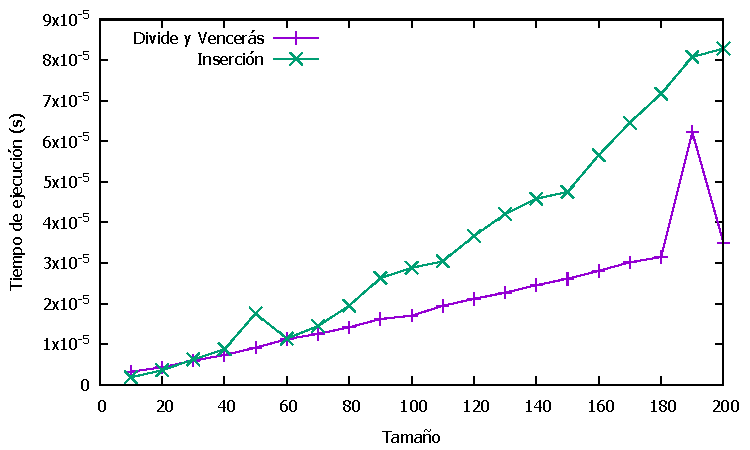
\includegraphics[width=14cm]{img/umbral_preferencias.pdf} \centering
	\caption{Tiempos según tamaño}
\end{figure}

El tiempo de ejecución del algoritmo basado en la ordenación por inserción se ajusta a la función $i(n) = 1.56413 \cdot 10^{-9} n^2 + 9.84525 \cdot 10^{-8} n + 2.08435 \cdot 10^{-6}$, mientras que el tiempo obtenido con el algoritmo derivado del \textit{mergesort} (ignorando el resultado obtenido en tamaño $190$) tiene por función de ajuste $m(n) = 3.08096 \cdot 10^{-8} n \cdot \log(n) + 3.07834 \cdot 10^{-6}$. \\

Esta gráfica compara las funciones de ajuste con los datos obtenidos:
\begin{figure}[H]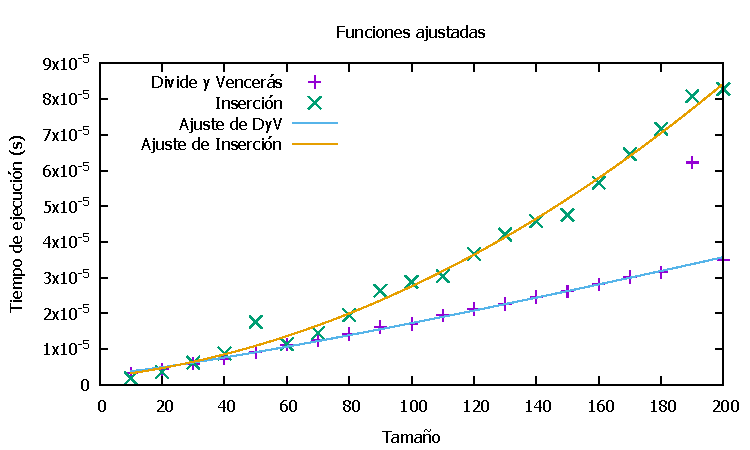
\includegraphics[width=14cm]{img/ajuste_preferencias.pdf} \centering
	\caption{Funciones de ajuste para determinar el umbral}
\end{figure}

Hallamos el punto de corte usando la función \texttt{find\_root} de Maxima:

\begin{lstlisting}[language=Maxima]
	i(n):=1.56413*10^(-9)*n^2 + 9.84525 * 10^(-8)*n + 2.08435*10^(-6)$
	m(n):=3.08096*10^(-8)*n*log(n) + 3.07834*10^(-6)$
	find_root(m(x)-i(x),x,10,200);
\end{lstlisting}

Obteniendo el punto de corte $25.726267$. Sin embargo, en pruebas posteriores de umbrales cercanos a ese punto de corte, hemos concluido que el umbral óptimo resultó estar alrededor de $50$.

\subsection{Comparación de algoritmos}

La tabla anterior recogía los tiempos obtenidos con el algoritmo basado en la ordenación por inserción y con el algoritmo basado en \textit{mergesort} con umbral $2$. En la siguiente tabla se completa con los tiempos obtenidos con el umbral considerado óptimo, $50$ (el número a continuación de \textit{Mergesort} es el umbral usado), y los tiempos con el algoritmo trivial:

\vspace*{1cm}

\pgfplotstableread{dats/preferencias_d.dat}\prefDVf
\pgfplotstableread{dats/preferencias_t.dat}\prefObv
\pgfplotstablecreatecol[copy column from table={\prefDVt}{[index] 1}] {par1} {\prefDVf}
\pgfplotstablecreatecol[copy column from table={\prefIns}{[index] 1}] {par2} {\prefDVf}
\pgfplotstablecreatecol[copy column from table={\prefObv}{[index] 1}] {par3} {\prefDVf}

\pgfplotstabletypeset[
display columns/0/.style={column name=Tamaño},
display columns/1/.style={column name=Mergesort $50$},
display columns/2/.style={column name=Mergesort $2$},
display columns/3/.style={column name=Inserción},
display columns/4/.style={column name=Algoritmo obvio},
]{\prefDVf}

\vspace*{1cm}

Que se ilustran con esta gráfica:

\begin{figure}[H]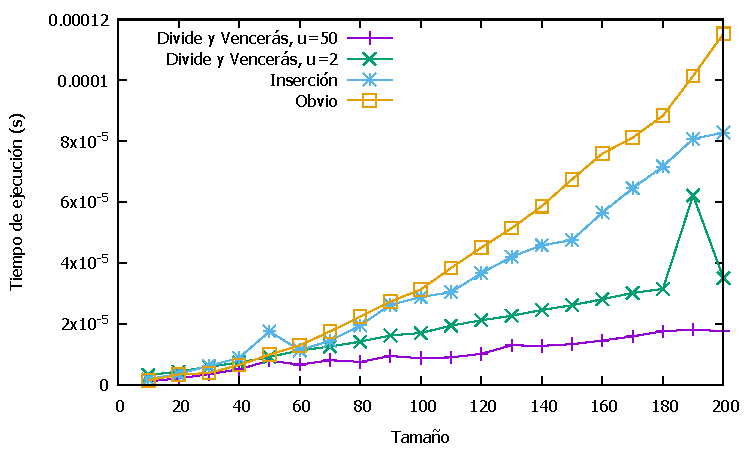
\includegraphics[width=14cm]{img/comparativa_preferencias.pdf} \centering
	\caption{Tiempos según tamaño para cada algoritmo}
\end{figure}

Además hemos repetido las ejecuciones con valores mayores para el algoritmo Divide y Vencerás con los dos umbrales, obteniendo esta tabla:

\vspace*{1cm}

\pgfplotstableread{dats/comp_umbral/preferencias_d_umbral.dat}\prefDVu
\pgfplotstableread{dats/comp_umbral/preferencias_d_sinumbral.dat}\prefDVs
\pgfplotstablecreatecol[copy column from table={\prefDVs}{[index] 1}] {par1} {\prefDVu}

\pgfplotstabletypeset[
display columns/0/.style={column name=Tamaño},
display columns/1/.style={column name=Mergesort $50$},
display columns/2/.style={column name=Mergesort $2$},
skip rows between index={25}{50}
]{\prefDVu}
\pgfplotstabletypeset[
display columns/0/.style={column name=Tamaño},
display columns/1/.style={column name=Mergesort $50$},
display columns/2/.style={column name=Mergesort $2$},
skip rows between index={0}{25}
]{\prefDVu}

\vspace*{1cm}

Y la gráfica siguiente:

\begin{figure}[H]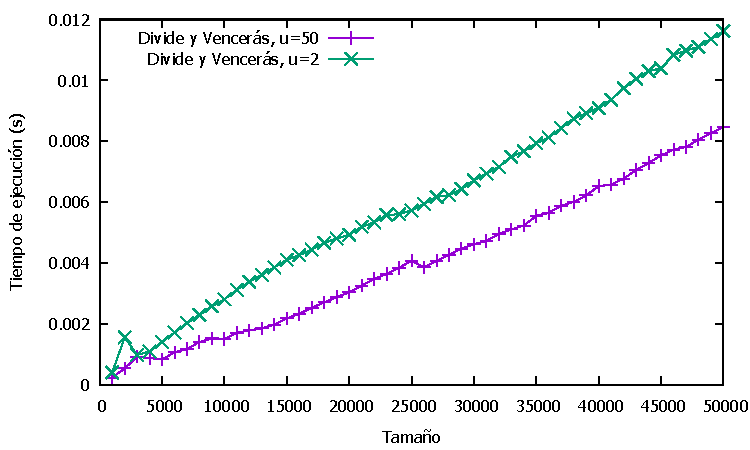
\includegraphics[width=14cm]{img/comparativa_preferencias_grande.pdf} \centering
	\caption{Tiempos según tamaño para Divide y Vencerás}
\end{figure}

Cabe destacar que los tiempos de ejecución del algoritmo trivial para valores en torno a $50\ 000$ se encuentran aproximadamente tres órdenes de magnitud por encima de los obtenidos para el algoritmo Divide y Vencerás con el umbral $50$.
